\documentclass[12pt]{article}
\usepackage{indentfirst}
\usepackage{url}
\usepackage{pgf-pie}

\setlength{\oddsidemargin}{27mm}
\setlength{\evensidemargin}{27mm}
\setlength{\hoffset}{-1in}

\setlength{\topmargin}{27mm}
\setlength{\voffset}{-1in}
\setlength{\headheight}{0pt}
\setlength{\headsep}{0pt}

\setlength{\textheight}{235mm}
\setlength{\textwidth}{155mm}

\pagestyle{plain}

\renewcommand{\thefootnote}{\fnsymbol{footnote}}
\renewcommand{\labelitemi}{$\bullet$}

\begin{document}
\baselineskip 11pt


\begin{center}
  \textbf{\Large Swaptor Whitepaper} \\

  \vspace{1.5cc}
  { \sc Marko Ivanković$^{1}$}\\

  \vspace{0.3 cm}

  {\small $^{1}$Berry Block, marko@berryblock.io}
\end{center}
\vspace{1.5cc}

\begin{abstract}
  \noindent  Peer-to-peer (P2P) swaps on blockchain have the potential to greatly benefit users by eliminating the need for intermediaries in the exchange of assets. However, the use of P2P swaps on blockchain also presents several challenges, including trust issues that must be addressed in order to ensure their success.  Since there is no intermediary to oversee the exchange of assets, users must rely on the trustworthiness of the other party to the transaction. In the absence of a trusted third party, it is difficult to verify the authenticity and quality of the assets being exchanged, which can lead to disputes and losses for users.
  \\ \indent Furthermore, P2P swaps on blockchain are subject to potential security risks, such as hacking and fraud. Since the transactions are conducted directly between users, there is a greater risk of malicious actors attempting to exploit vulnerabilities in the system. This risk is exacerbated by the fact that blockchain transactions are irreversible, meaning that users have no recourse if their assets are stolen or lost.
  \\ \indent In this paper we describe Swaptor, a decentralized P2P exchange dapp which aims to eliminate problems mentioned above.

  \vspace{0.95cc}
\end{abstract}

\newpage

\tableofcontents

\newpage

\section{Architectural Overview} \label{form}
\indent As most modern dapps, Swaptor's architecture is a mix of on-chain and off-chain components:
\begin{itemize}
  \item \textbf{On-chain}: Smart contracts
  \item \textbf{Off-chain}: Backend, Frontend and Database
\end{itemize}

\subsection{On-chain Architecture}

\indent Smart contracts are written in Solidity, and their architecture is designed to be minimalistic.
Specifically, the Swaptor contract is a singular entity whose sole purpose is to verify digital signatures
and execute swaps upon successful verification. Digital signatures encode the specific terms under which a given swap is considered valid.

\subsubsection{Signatures}

In order to verify the signature, the smart contract must possess both the original swap elements
and the signature itself. Prior to being passed as an argument to one of the \textit{acceptSwap} functions,
these elements are encoded using the \textit{abi.encode} function. The signature is generated by creating a
\textit{keccak256} hash of the encoded arguments and signing it with the private key belonging to the seller.
This method dramatically reduces the gas fees because the seller never had to transfer their assets to Swaptor contract.

\subsubsection{Swap types}

At present, Swaptor facilitates the swapping of ERC-721 and ERC-20 tokens, enabling the execution of any combination of swaps involving these types of tokens.
In the future, Swaptor intends to extend its support to include native currency and ERC-1155 tokens.

\subsubsection{Fees}
To accept the swap, an address will need to pay a fixed fee of \$$5$ in the native currency, which is calculated using Chainlink oracles\cite{chainlink}. It should be noted that the fee is not fixed and may be subject to change.

\subsection{Off-chain Architecture}

\subsubsection{Backend}

\subsubsection{Frontend}

\subsubsection{Database \& Security}

\section{Tokenomics}

\subsection{Token Allocation}

\begin{figure}[h]
  \centering
  \begin{tikzpicture}
    \pie{34/Public sale, 22/VC, 16/Team, 18/Community, 10/Liquidity pool}
  \end{tikzpicture}
  \caption{Pie chart showing the distribution of tokens}
  \label{fig:pie-chart}
\end{figure}

\section{Roadmap}
\dots

\begin{thebibliography}{9}
  \bibitem{chainlink} What is an oracle in blockchain? explained | chainlink, \url{https://chain.link/education/blockchain-oracles}
\end{thebibliography}

\end{document}